% !Mode:: "TeX:UTF-8"

\chapter{经典语音识别HMM-GMM基本原理}\label{intro_hmm}

现今的连续语音识别系统大多采用隐马尔可夫模型HMM\ucite{rabiner1989tutorial,huang2001spoken,bishop2006pattern}。隐马尔科夫模型(HMM)是一种统计模型,
已广泛应用于语音信号处理的各个领域中。HMM的理论基础是在二十世纪七十年代由Baum等人建立起来的,在之后的发展
中被Baker和Jelinek等人应用于语音识别中,并取得了巨大成功。目前,其基本理论和各种实用算法是现代语音识别研究
的重要方向之一。

本章介绍基于隐马尔可夫模型HMM的语音识别的基本原理。

\newtheorem{definition}{\hspace{2em}\textbf{定义}}[section]
%\newtheorem{algorithm}{\hspace{2em}\textbf{算法}}[section]
%
%\section{隐马尔科夫模型的概念\cite{lihang2012}}
%    \begin{definition}[隐马尔科夫模型]
%    隐马尔科夫模型是关于时序的概率模型,描述由一个隐藏的马尔科夫链随机生成不可观测的状态序列,再由各个状态生成
%    一个观测而产生观测序列的过程。隐藏的马尔科夫链随机生成的状态的序列,称为状态序列(state sequence);每个状态
%    生成一个观测,而由此产生的观测的随机序列,称为观测序列(observation sequence)。
%    \end{definition}
%
%
%    隐马尔科夫模型由初始概率分布,状态转移概率分布以及观测概率分布确定,隐马尔科夫模型的形式定义如下:
%
%    设$Q$是所有可能的状态的集合,$V$是所有可能的观测的集合。
%    \[Q = \{ {q_1},{q_2},\cdots,{q_N}\} , V = \{ {v_1},{v_2},\cdots,{v_M}\} \]
%    其中,$N$是可能的状态数,$M$是可能的观测数。
%
%    $I$是长度为T的状态序列,$O$是对应的观测序列。
%    \[I = ({i_1},{i_2},\cdots,{i_T}), O = ({o_1},{o_2},\cdots,{o_T})\]
%
%    $A$是状态转移矩阵:
%    \begin{equation}
%    A = {\left[ {{a_{ij}}} \right]_{N \times N}}
%    \end{equation}
%    其中,
%    \begin{equation}
%    {a_{ij}} = {\kern 1pt} P({i_{t + 1}} = {q_j}|{i_t} = {q_i}),{\kern 1pt} {\kern 1pt} i = 1,2, \cdots ,N;{\kern 1pt} j = 1,2, \cdots ,N
%    \end{equation}
%    是在时刻$t$处于状态$q_i$的条件下在时刻$t+1$转移到状态$q_j$的概率。
%
%    $B$是观测概率矩阵:
%    \begin{equation}
%    B = {\left[ {{b_{j}(k)}} \right]_{N \times M}}
%    \end{equation}
%    其中,
%    \begin{equation}
%    {b_{j}(k)} = {\kern 1pt} P({o_t} = {v_k}|{i_t} = {q_j}),{\kern 1pt} {\kern 1pt} k = 1,2, \cdots ,N;{\kern 1pt} j = 1,2, \cdots ,N
%    \end{equation}
%    是在时刻$t$处于状态$q_j$的条件下生成观测$v_k$的概率。
%
%    $\pi$是初始状态概率向量:
%    \begin{equation}
%    \pi  = ({\pi _i})
%    \end{equation}
%    其中,
%    \begin{equation}
%    {\pi _i} = P({i_1} = {q_i}),i = 1,2, \cdots N
%    \end{equation}
%    是时刻$t=1$处于状态$q_i$的概率。
%
%    隐马尔科夫模型由初始状态概率向量$\pi$、状态转移概率矩阵$A$和观测概率矩阵$B$决定,$\pi$和$A$决定状态序列。因此,隐马尔科夫模型$\lambda $
%    可以用三元符号表示,即
%    \begin{equation}
%    \lambda  = \left( {A,B,\pi } \right)
%    \end{equation}
%    ${A,B,\pi }$称为隐马尔科夫模型的三要素。
%
%    状态转移概率矩阵$A$与初始状态概率向量$\pi$确定了隐藏的马尔科夫链,生成不可观测的状态序列。观测概率矩阵$B$确定了如何从状态生成观测,与状态序列
%    综合确定了如何产生观测序列。
%
%    从定义可知,隐马尔科夫模型做了两个基本的假设:
%    \vspace{-10pt}
%    \begin{enumerate}
%    	\item 齐次马尔科夫性假设,即假设隐藏的马尔科夫链在任意时刻$t$的状态只依赖于前一时刻的状态,与其他时刻的状态与观测无关,也与时刻$t$无关。
%            \begin{equation}
%            P({i_t}|{t_{t - 1}},{o_{t - 1,}} \cdots {i_1},{o_1}) = P({i_t}|{i_{t - 1}}),t = 1,2, \cdots T
%            \end{equation}
%        \item 观测独立性假设,及假设任意时刻的观测只依赖于该时刻的马尔科夫链的状态,与其他观测及状态无关。
%            \begin{equation}
%            P({o_t}|{t_T},{o_{T,}} \cdots ,{i_t},{o_t}, \cdots ,{i_1},{o_1}) = P({o_t}|{i_t})
%            \end{equation}
%    \end{enumerate}
%    \vspace{-10pt}
%
%\section{HMM的三个基本问题\cite{lihang2012}}
%    隐马尔科夫模型有3个基本问题:
%    \vspace{-10pt}
%    \begin{enumerate}
%        \item 概率计算问题。给定模型$\lambda  = \left( {A,B,\pi } \right)$和观测序列$O = ({o_1},{o_2},\cdots,{o_T})$,计算在模型$\lambda$下观测
%            序列$O$出现的概率$P(O|\lambda )$。
%        \item 学习问题。已知观测序列$O = ({o_1},{o_2},\cdots,{o_T})$,估计模型$\lambda  = \left( {A,B,\pi } \right)$参数,使得在该模型下观测序列
%            概率$P(O|\lambda )$最大。即用最大似然估计的方法估计参数。
%        \item 预测问题,也称解码问题。已知模型$\lambda  = \left( {A,B,\pi } \right)$和观测序列$O = ({o_1},{o_2},\cdots,{o_T})$,求对给定观测序列
%            条件概率$P(I|O)$最大的状态序列$I = ({i_1},{i_2},\cdots,{i_T})$。即给定观测序列,求最有可能的对应状态序列。
%    \end{enumerate}
%    \vspace{-10pt}
%
%    \subsection{概率问题}\label{section:probability}
%    本节介绍计算观测序列概率$P(O|\lambda )$的前向算法与后向算法,为方便后面计算学习问题,结合前向后向算法,本节第三小节定相关数学符号。
%        \subsubsection{前向算法}
%        \begin{definition}[前向算法]
%            给定隐马尔科夫模型$\lambda$,定义到时刻$t$部分观测序列为$({o_1},{o_2},\cdots,{o_T})$且状态为$q_i$的概率为前向概率,记作
%            \begin{equation}
%            {\alpha _t}(i) = P({o_1},{o_2}, \cdots {o_t},{i_t} = {q_i}|\lambda )
%            \end{equation}
%        \end{definition}
%
%        则可递推地求得前向概率${\alpha _t}(i)$及观测序列概率$P(O|\lambda )$,算法描述如下:
%        \begin{enumerate}
%            \item 初值
%                \begin{equation}
%                    {\alpha _1}(i) = {\pi _i}{b_i}({o_1}),i = 1,2, \cdots N
%                \end{equation}
%            \item 前向递推~~~~对$t = 1,2, \cdots ,T - 1$,如图\ref{fig:forback},
%                \begin{equation}
%                    {\alpha _{t + 1}}(i) = \left[ {\sum\limits_{j = 1}^N {{\alpha _t}(j){a_{ji}}} } \right]{b_i}({o_{t + 1}}),i = 1,2, \cdots ,N
%                \end{equation}
%            \item 终止
%                \begin{equation}
%                    P(O|\lambda ) = \sum\limits_{i = 1}^N {{\alpha _T}(i)}
%                \end{equation}
%        \end{enumerate}
%
%        \begin{figure}
%        \centering
%        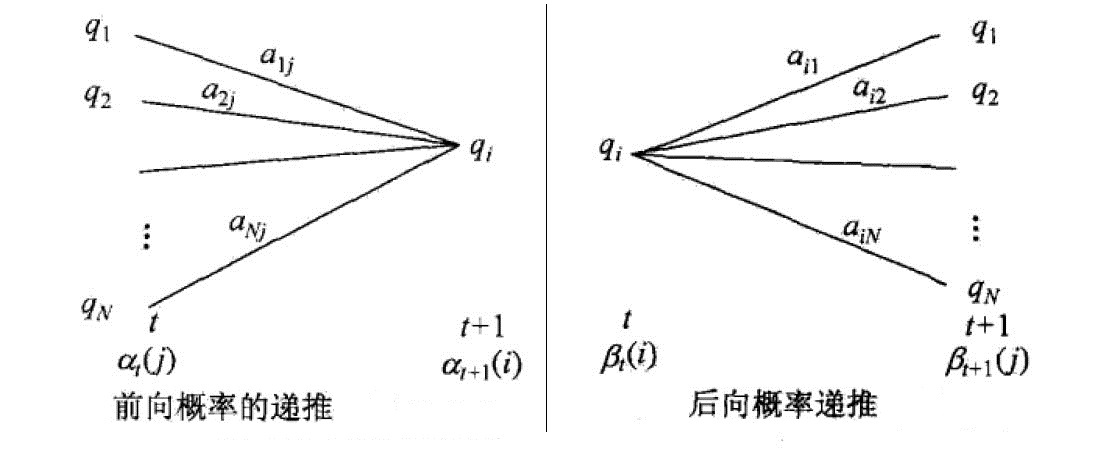
\includegraphics[width=0.9\textwidth]{figures/forback}
%        \caption{前向后向概率计算示意图}
%        \label{fig:forback}
%        \end{figure}
%
%        \subsubsection{后向算法}
%        \begin{definition}[后向算法]
%         给定隐马尔科夫模型$\lambda$,定义在时刻$t$状态为$q_i$的条件下,从$t+1$到$T$的部分观测序列为$({o_{t+1}},{o_{t+2}},\cdots,{o_T})$的概率为后向概率,记作
%             \begin{equation}
%                 {\beta _t}(i) = P({o_{t + 1}},{o_{t + 2}}, \cdots ,{o_T}|{i_t} = {q_i},\lambda )
%             \end{equation}
%        \end{definition}
%
%        则可递推地求得后向概率${\beta _t}(i)$及观测序列概率$P(O|\lambda )$,算法描述如下:
%        \begin{enumerate}
%            \item 初值
%                \begin{equation}
%                    {\beta _T}(i) = 1,i = 1,2, \cdots ,N
%                \end{equation}
%            \item 后向递推,对于$t = T - 1,T - 2, \cdots ,1$,如图\ref{fig:forback},
%                 \begin{equation}
%                    {\beta _t}(i) = \sum\limits_{j = 1}^N {{a_{ij}}{b_j}({o_{t + 1}}){\beta _{t + 1}}(j),i = 1,2, \cdots N}
%                 \end{equation}
%            \item 终止
%                \begin{equation}
%                    P(O|\lambda ) = \sum\limits_{i = 1}^N {{\pi _i}{b_i}({o_1}){\beta _1}\left( i \right)}
%                \end{equation}
%        \end{enumerate}
%
%        \subsubsection{新数学符号定义}
%        利用前向概率和后巷概率,我们引出以下概念
%        \begin{enumerate}
%            \item 观测序列概率$P(O|\lambda )$的统一形式:
%                \begin{equation}
%                    P(O|\lambda ) = \sum\limits_{i = 1}^N {\sum\limits_{j = 1}^N {{\alpha _t}(i)} {a_{ij}}{b_j}({o_{t + 1}}){\beta _{t + 1}}\left( j \right),} t = 1,2, \cdots T - 1
%                \end{equation}
%            \item 给定模型$\lambda $和观测$O$,在时刻$t$处于状态$q_i$的概率,记
%                \begin{equation}
%                    {\gamma _t}(i) = P({i_t} = {q_i}|O,\lambda )
%                \end{equation}
%                可以通过前向后向概率计算。事实上,
%                \[{\gamma _t}(i) = P({i_t} = {q_i}|O,\lambda ) = \frac{{P({i_t} = {q_i},O|\lambda )}}{{P(O|\lambda )}}\]
%                由前向后向概率定义可知:
%                \[{\alpha _t}(i){\beta _t}(i) = P({i_t} = {q_i},O|\lambda )\]
%                如图\ref{fig:gamma},于是有:
%                \begin{equation}\label{equation:gamma}
%                {\gamma _t}(i) = \frac{{{\alpha _t}(i){\beta _t}(i)}}{{P(O|\lambda )}} = \frac{{{\alpha _t}(i){\beta _t}(i)}}{{\sum\limits_{j = 1}^N {{\alpha _t}(j){\beta _t}(j)} }}
%                \end{equation}
%
%                \begin{figure}
%                \centering
%                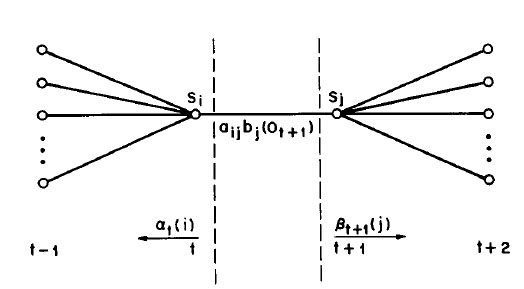
\includegraphics[width=0.7\textwidth]{figures/gamma}
%                \caption{${\gamma _t}(i)$计算示意图}
%                \label{fig:gamma}
%                \end{figure}
%
%            \item 定模型$\lambda $和观测$O$,在时刻$t$处于状态$q_i$且在$t+1$时刻处于状态$q_j$的概率记作
%                \begin{equation}
%                    {\xi _t}(i,j) = P({i_t} = {q_i},{i_{t + 1}} = {q_j}|O,\lambda )
%                \end{equation}
%                通过前向后向概率计算得:
%                \[{\xi _t}(i,j) = \frac{{P({i_t} = {q_i},{i_{t + 1}} = {q_j},O|\lambda )}}{{P(O|\lambda )}} = \frac{{P({i_t} = {q_i},{i_{t + 1}} = {q_j},O|\lambda )}}{{\sum\limits_{i = 1}^N {\sum\limits_{j = 1}^N {P({i_t} = {q_i},{i_{t + 1}} = {q_j},O|\lambda )} } }}\]
%                而
%                \[P({i_t} = {q_i},{i_{t + 1}} = {q_j},O|\lambda ) = {\alpha _t}(i){a_{ij}}{b_j}({o_{t + 1}}){\beta _{t + 1}}(j)\]
%                所以
%                \begin{equation}\label{equation:xi}
%                {\xi _t}(i,j) = \frac{{{\alpha _t}(i){a_{ij}}{b_j}({o_{t + 1}}){\beta _{t + 1}}(j)}}{{\sum\limits_{i = 1}^N {\sum\limits_{j = 1}^N {{\alpha _t}(i){a_{ij}}{b_j}({o_{t + 1}}){\beta _{t + 1}}(j)} } }}
%                \end{equation}
%        \end{enumerate}
%    \subsection{学习问题}\label{section:learn}
%        假设给定训练数据只包含$S$个长度为T的观测序列$\{ {O_1},{O_2}, \cdots ,{O_s}\} $而没有对应的状态序列,目标是学习隐马尔科夫模型$\lambda  = \left( {A,B,\pi } \right)$的参数。我们将观测序列数据看做观测数据$O$,状态序列数据看作不可观测的隐数据$I$,那么隐马尔科夫模型事实上是一个含有隐变量的概率
%        模型
%        \begin{equation}
%        P(O|\lambda ) = \sum\limits_I {P(O|I,\lambda )P(I|\lambda )}
%        \end{equation}
%        它的学习参数学习可以由EM算法实现。
%
%        EM算法是一种迭代算法,1977年由Dempster等人总结提出,用于含有隐变量的概率模型参数的极大似然估计,或极大后验估计。EM算法每次迭代由两步组成:E步,求期望
%        (expectation);M步,求极大(maximization)。所以这一算法称为期望极大算法(expectation maximization algorithm),简称EM算法。下面直接给出Baum-Welch算法,由Baum和Welch提出,是EM算法在隐马尔科夫模型学习中的具体实现。
%
%
%        \begin{algorithm}[Baum-Welch算法]Baum-Welch算法输入为观测数据$O = \{ {o_1},{o_2}, \cdots ,{o_T}\}$,输出为隐马尔科夫模型参数。算法步骤如下:
%            \begin{enumerate}
%                \item 初始化
%
%                    对于$n=0$,选取$a_{ij}^{(0)}$,${b_j}{(k)^{(0)}}$,$\pi _i^{(0)}$,得到模型${\lambda ^{(0)}} = \left( {{A^{(0)}},{B^{(0)}},{\pi ^{(0)}}} \right)$。
%                \item 递推,对于$n = 1,2, \cdots $,
%                    \[a_{ij}^{(n + 1)} = \frac{{\sum\limits_{t = 1}^{T - 1} {{\xi _t}(i,j)} }}{{\sum\limits_{t = 1}^{T - 1} {{\gamma _t}(i)} }}\]
%                    \[{b_j}{(k)^{(n + 1)}} = \frac{{\sum\limits_{t = 1,{o_t} = {v_k}}^T {{\gamma _t}(j)} }}{{\sum\limits_{t = 1}^T {{\gamma _t}(j)} }}\]
%                    \[\pi _i^{(n + 1)} = {\gamma _1}(i)\]
%                    右端各值按观测$O = \{ {o_1},{o_2}, \cdots ,{o_T}\}$和模型${\lambda ^{(n)}} = \left( {{A^{(n)}},{B^{(n)}},{\pi ^{(n)}}} \right)$计算。
%                    式中${{\gamma _t}(j)}$和${{\xi _t}(i,j)}$由式\ref{equation:gamma}和式\ref{equation:xi}给出。
%               \item 终止。得到模型参数${\lambda ^{(n + 1)}} = \left( {{A^{(n + 1)}},{B^{(n + 1)}},{\pi ^{(n + 1)}}} \right)$。
%            \end{enumerate}
%        \end{algorithm}
%
%    \subsection{预测问题}\label{section:predict}
%    隐马尔科夫模型的预测问题可以由维特比算法(Viterbi算法)解决,下面给出维特比算法。
%
%    维特比算法实际是用动态规划解隐马尔科夫模型预测问题,即用动态规划求最大概率路径(最优路径)。这时求解出的一条路径对应一个状态序列。
%
%    根据动态规划原理,最优路径具有这样的特性;如果最优路径在时刻$t$通过节点${i_t}^*$,那么这一路径从节点${i_t}^*$到终点${i_T}^*$的部分路径,
%    对于从${i_t}^*$到${i_T}^*$的所有可能的部分路径来说,必须是最优的。因为如果不是这样,那么从${i_t}^*$到${i_T}^*$就有另一条更好的部分路径
%    存在,如果把它和从${i_1}^*$到达${i_t}^*$的部分路径连接起来,就会形成比原来路径更优的路径,这是矛盾的。依据这一原理,我们只需从$t=1$时刻
%    开始,递推地计算在时刻$t$状态为$i$的各条部分路径的最大概率,直至得到时刻$t=T$状态为$i$的各条路径的最大概率。时刻$t=T$的最大概率即为最大
%    概率即为最有路径的概率${P^*}$,最优路径的终结点${i_T}^*$也同时得到。之后,为了找出最优路径的各个节点,从终结点${i_T}^*$开始,由后向前逐步
%    求得节点${i_{T - 1}}^*, \cdots ,{i_1}^*$,得到最优路径${I^*} = ({i_1}^*,{i_2}^*, \cdots ,{i_{T - 1}}^*,{i_T}^*)$,这就是维特比算法。
%
%    算法首先导入两个变量$\delta $和$\psi $。定义在时刻$t$状态为$i$的所有单个路径$({i_1},{i_2}, \cdots ,{i_t})$中概率最大值为
%        \begin{equation}
%            {\delta _t}(i) = \mathop {\max }\limits_{{i_1},{i_2}, \cdots ,{i_{t - 1}}} P({i_t} = i,{i_{t - 1}}, \cdots ,{i_1},{o_t}, \cdots ,{o_1}|\lambda ),i = 1,2,, \cdots ,N
%        \end{equation}
%
%    由定义可得变量$\delta $的递推公式:
%        \begin{equation}
%            \begin{array}{l}
%            {\delta _{t + 1}}(i) = \mathop {\max }\limits_{{i_1},{i_2}, \cdots ,{i_t}} P({i_{t + 1}} = i,{i_t}, \cdots ,{i_1},{o_{t + 1}}, \cdots ,{o_1}|\lambda )\\
%            \;\;\;\;\;\;\;\;\; = \mathop {\max }\limits_{1 \le j \le N} \left[ {{\delta _t}(j){a_{ji}}} \right]{b_i}({o_{t + 1}}),i = 1,2, \cdots ,N;t = 1,2, \cdots,T - 1
%        \end{array}
%        \end{equation}
%
%    定义在时刻$t$状态为$i$的所有单个路径$({i_1},{i_2}, \cdots ,{i_t})$中概率最大的路径第$t-1$个节点为:
%         \begin{equation}
%            {\psi _t}(i) = arg\mathop {\max }\limits_{1 \le j \le N} [{\delta _{t - 1}}(j){a_{ji}}],i = 1,2, \cdots, N
%        \end{equation}
%
%    \begin{algorithm}[Viterbi算法]算法输入为观测数据$O = \{ {o_1},{o_2}, \cdots ,{o_T}\}$和模型参数$\lambda  = \left( {A,B,\pi } \right)$,输出为最优路径${I^*} = ({i_1}^*,{i_2}^*, \cdots ,{i_{T - 1}}^*,{i_T}^*)$。算法步骤如下:
%        \begin{enumerate}
%                \item 初始化
%                    \[{\delta _1}(i) = {\pi _i}{b_i}({o_1}),i = 1,2, \cdots ,N\]
%                    \[{\psi _1}(i) = 0,i = 1,2, \cdots ,N\]
%                \item 递推,对于$t = 1,2, \cdots,T$,
%                    \[{\delta _t}(i) = \mathop {\max }\limits_{1 \le j \le N} \left[ {{\delta _{t - 1}}(j){a_{ji}}} \right]{b_i}({o_t}),i = 1,2, \cdots ,N\]
%                    \[{\psi _t}(i) = arg\mathop {\max }\limits_{1 \le j \le N} [{\delta _{t - 1}}(j){a_{ji}}],i = 1,2, \cdots ,N\]
%                \item 终止
%                    \[{P^*} = \mathop {\max }\limits_{1 \le i \le N} {\delta _T}(i)\]
%                    \[{i_T}^* = arg\mathop {\max }\limits_{1 \le i \le N} \left[ {{\delta _T}(i)} \right]\]
%                \item 最优路径回溯。对于$t = T-1,T-2, \cdots,1$
%                    \[{i_t}^* = {\psi _{t + 1}}({i_{t + 1}}^*)\]
%                    从而求得最优路径${I^*} = ({i_1}^*,{i_2}^*, \cdots ,{i_{T - 1}}^*,{i_T}^*)$
%        \end{enumerate}
%    \end{algorithm}
%
%
%\section{连续密度的隐马尔科夫模型\cite{zhaoli2009}}
%
%    以上讨论中,我们都假定观测输出概率,也就是$B$参数的分布是离散的,本节介绍连续密度的隐马尔科夫模型(Continuous HMM,CHMM)。
%    在连续密度隐马尔科夫模型中,观测输出概率是连续的,而不是有限的,所以不能用观测矩阵来表示输出概率,而要改用概率密度函数来表示。
%    假设$\bm{X}$为观测向量,则$[b_{j}(\bm{X})d\bm{X}]$表示在$\bm{X}$和$\bm{X}+d\bm{X}$之间观察矢量的输出概率。这里$b_{j}(\bm{X})$
%    称为参数$\bm{X}$的概率密度分布函数,输出$\bm{X}$的概率可以通过$b_{j}(\bm{X})$计算。$b_{j}(\bm{X})$一般用高斯概率密度函数,由于
%    $\bm{X}$是多维矢量,所以要用多元高斯密度函数,如式\ref{equation:gm}所示。
%    \begin{equation}\label{equation:gm}
%       {b_j}(\bm{X}) = \frac{1}{{{{(2\pi )}^{p/2}}{|{\bm{\Sigma}} |_j^{ - 1}}}}\exp \left\{ { - \frac{1}{2}(\bm{X} - {{\bm{\mu}} _j}) {\bm{\Sigma}}_j^{ - 1}{{(\bm{X} - {{\bm{\mu}}_j})}^T}} \right\}
%    \end{equation}
%
%    另一方面,在实际应用中,仅用一个高斯概率密度函数不足以表述语音参数$\bm{X}$的输出概率分布,所以常用多个高斯函数的叠加组合来表示输出概率
%    密度函数,称为混合高斯模型,如式\ref{equation:gmm}所示。
%    \begin{equation}\label{equation:gmm}
%       {b_j}(\bm{X}) = \sum\limits_{m = 1}^M {{\omega _{jm}}} \frac{1}{{{{(2\pi )}^{p/2}}|{\bm{\Sigma}} |_{jm}^{ - 1}}}\exp \left\{ { - \frac{1}{2}(\bm{X} - {{\bm{\mu}} _{jm}}){\bm{\Sigma}}_{jm}^{ - 1}{{(\bm{X} - {{\bm{\mu}} _{jm}})}^T}} \right\}
%    \end{equation}
%
%    其中$M$表示混合高斯数,即使用$M$个高斯叠加组合描述输出概率密度函数,${\omega_{jm}}$是混合系数,表示第$m$个高斯所占权重。混合高斯的引入,极大的增强了模型
%    的描述能力。
%
%
%\section{HMM在语音识别中的应用}
%    结合HMM的三个基本问题和连续密度的HMM,本节介绍HMM在语音识别中的模型建立、训练过程和识别过程的基本应用。
%
%    首先,要明确在语音识别任务中观测是什么、状态是什么。观测是人所发出的一段语音信号,人在说不同词时会产生不同的语音信号,不同的语音信号对应不同的信号特征(
%    如幅度、频率、过零率等),我们对语音信号进行特征提取,即可作为HMM模型的观测向量,本毕设中使用39维MFCC特征。人在发出不同音素时对应不同的发音过程,状态即是对
%    不同发音过程的描述。由于人的发音过程不可逆,即状态跳转不可逆,语音识别任务中使用特殊的HMM模型,称为左右模型,如图\ref{fig:left_right}所示,可以看出仅能跳转到
%    自身或更高的状态。若以音素为基本单位建立HMM模型,则一般使用3状态的HMM描述,如图\ref{fig:asr_hmm}所示,其中1、5状态为扩展状态,1状态为起始状态,只能跳转到其它
%    状态;5状态为结束状态。1、5状态均不产生任何观测输出,只是为了描述的方便,特别在HMM模型连接中非常有用。
%
%    \begin{figure}
%    \centering
%    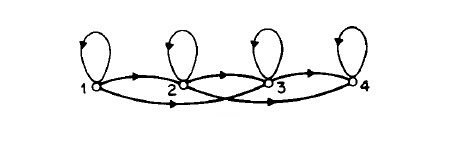
\includegraphics[width=0.8\textwidth]{figures/left_right}
%    \caption{左右模型HMM}
%    \label{fig:left_right}
%    \end{figure}
%
%    \begin{figure}
%    \centering
%    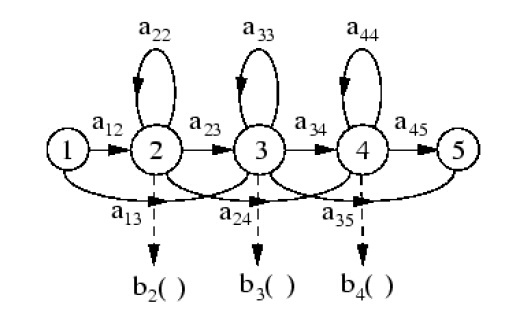
\includegraphics[width=0.8\textwidth]{figures/asr_hmm}
%    \caption{语音识别中的5状态HMM}
%    \label{fig:asr_hmm}
%    \end{figure}
%
%    模型的训练是一个不断迭代的过程,目的是求得各个HMM模型的参数。准备好数据,包括语音特征文件(39维MFCC特征)和标注后。
%    以音素为基本单位的训练过程如下:
%    首先,对每个音素建立一个HMM模型,并对模型参数$\lambda $进行初始化。
%    每一轮的训练过程中,根据HMM模型参数,先使用前向后向算法计算(HMM概率问题\ref{section:probability})在所有时间$t$上的前向得分和后向得分,随后进行Baum-Welch
%    算法(HMM学习问题\ref{section:learn})对模型参数进行更新,其中E步计算观测下各状态出现、各状态转移、由状态$i$转移到状态$j$的期望,并计算混合高斯分量权重的期望,
%    M步对状态转移矩阵,各状态概率密度函数混合高斯的均值、协方差矩阵参数进行更新。
%    重复进行训练过程,直至满足预设条件终止。
%
%    在已经得到各个HMM的模型参数后,识别过程就是计算给定观测在不同HMM模型上的概率,选取概率最大HMM模型对应的建模单元(如音素或词)即为识别结果。此时
%    即可以使用前向或者后向算法(HMM概率问题\ref{section:probability})计算概率,也可使用Viterbi算法(HMM预测问题\ref{section:predict})。然而,往往
%    还希望得到识别结果所对应的观测序列,因此一般使用Viterbi算法。在大词汇量连续语音识别中,为了提高识别的实时性,会采取措施限制识别任务的搜索空间,如
%    HVite中的Token Passing\cite{young1989token}算法和Beam剪枝策略。

%\section{基于HTK的连续语音识别系统}
%    \subsection{HTK工具包介绍}
%
%    HTK(HMM Tools Kit)\cite{young1997htk}是一个剑桥大学开发的专门用于建立和处理HMM的实验工具包,主要应用于语音识别领域,也可以应用于语音合成、字符识别和
%    DNA排序等领域。HTK经过剑桥大学、Entropic公司及Microsoft公司的不断增强和改进,使其在世界范围内得到广泛应用。并且,HTK源代码开放,
%    基于ANSI C实现,所以具有良好可移植性和跨平台性。HTK由库程序和工具程序两部分组成。库程序提供一系列函数和接口;工具程序为语音分析,
%    HMM训练、测试和结果分析提供一系列实现。
%
%    其中本毕设中主要使用HTK核心模块HEREST(训练工具)和HVite(识别工具)。
%
%
%    \subsection{HTK连续语音识别系统搭建}
%    \begin{figure}[h]
%        \centering
%        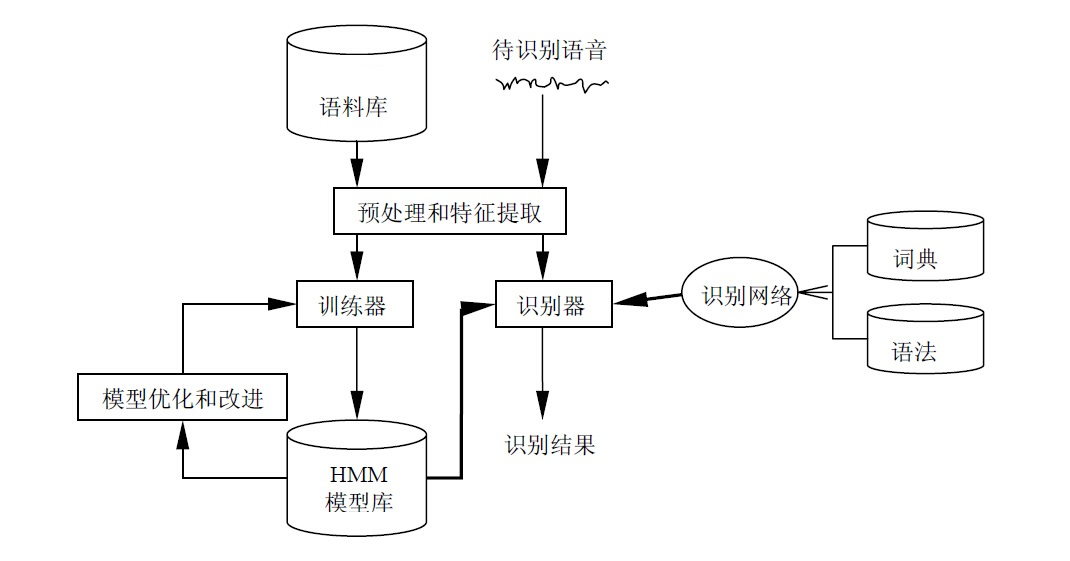
\includegraphics[width=0.8\textwidth]{figures/asr_system}
%        \caption{连续语音识别系统框架}
%        \label{fig:asr_system}
%    \end{figure}
%
%    一个连续语音识别系统架构如图\ref{fig:asr_system}所示,由图可以看出,整个系统由训练和识别两大部分组成,在HTK中其对应核心实现部分为HEREST和HVite。
%
%    本节介绍基于HTK连续语音识别系统搭建的数据准备、模型训练和识别系统。
%
%    数据准备部分主要准备字典、词典和语音数据及其对应标注抄本。本毕设中主要依托实验室的资源。
%
%    模型训练过程为:对语音数据进行特征提取;创建单音素模型;加入上下文信息创建三音素模型,三音素模型状态绑定,最后对HMM模型逐步增加混合高斯数。
%    训练过程中重复使用到HEREST。
%
%    识别系统首先定义任务所需的词网络,根据训练过程中产生的模型文件,先对输入语音进行特征提取,然后由识别器词网络在上根据声学模型和语言模型进行打分,进而
%    得到识别结果。识别过程核心为HVite,为了移植HVite到DSP,本毕设对HVite源代码进行了解析。

